\section{Introduction}\label{introduction}


The concept of 'Knowledge' has been the topic of extensive research for many
centuries for scientists and philosophers. For a Cognitive System, knowledge
provides the basic blocks on which the system will function. The Cognitive
Systems itself is incapable of taking in new data and without the knowledge of
previous actions and works, it can not learn and produce results.

Data, being a major part of knowledge, and it's type will indicate what type of
methods and algorithms are needed to build a particular Cognitive System.

\begin{itemize}
	\item For example, if the system is provided with text-based data, then some key
	      features that the machine learning will have to consider includes- sentiment
	      analysis, PoS Tagging, identification and analysis of non-conventional text
	      forms like emojis, etc. Natural Language Processing (NLP) techniques extract
	      the meaning from a given text by identifying the grammar and it's various rules
	      and using it to uncover the meaning behind the text. Linguistic Analysis helps
	      in breaking down the text in order to get the meaning behind it.
\end{itemize}

\begin{itemize}
	\item For Image based data, some key machine learning techniques include Principle
	      Component Analysis (PCA), developed by Kirby and Servich in the late 1980s;
	      Eigenface-Fisher Linear Discriminant (EFLD) and Dynamic Fuzzy Neural Networks
	      (DFNN). The latter two algorithms are extensively used in face recognition, in
	      terms of identifying dimensions of facial features. In recent times, Facebook
	      has come up with it's own face recognition software DeepFace.
\end{itemize}

\begin{itemize}
	\item For Speech based data, various stochastic models and Hidden Markov Model(HMM)
	      have been used, especially for solving the problem of Automatic Speech
	      Recognition. Nowadays, Automated Speech Recognition is widely in talks due to
	      it's ability to identify patterns and recognise the context and meaning behind
	      the speech. As technology further progresses, Speech Analysis becomes more and
	      more important.
\end{itemize}
For a Cognitive System to be able to have 'Cognition' and be a part of the society, it is imperative to build the system so that it can capture and assess knowledge like humans, so that it can make it's own decisions on it's own.

\section{The Importance of Knowledge in Cognitve Systems}\label{The Importance of Knowledge in Cognitive Systems}

History of Knowledge has become a discipline of itself, getting it's presence
acknowledged since the 2000s, with the advent of the internet and later Big
Data. The already existing knowledge and it's applications have been helpful
for scientists to build further theories and also to rectify or challenge
already existing models. This is the way our civilisation has been able to
produce all the scientific and technological marvels.


The Cognitive System is expected to function in a similar fashion. The
Cognitive System, depending on whether it utilises Supervised or Unsupervised
Learning, will require external sources to able to perform it's tasks, whether
it be predicting future outcomes, being able to provide solutions to everyday
problems.


Taking the example of current AI tools like Gemini and ChatGPT, which utilise
the enormous collection of data present on the internet, alongside it's
efficient learning algorithms which not only allows them to provide answers to
questions and hold on a full-fledged conversations, but also allows them to
rectify the errors made by them in future.


All this requires an extensive and sophisticated collection and management of
existing data. This is where Knowledge Representation comes in. The various
methods involved in Knowledge Representation are essential in providing the
Cognitive System a clear picture of the current situation and also to learn
further.

Knowledge in Cognitive Systems is what allows it function efficiently. Without
knowledge from external sources, most of the systems would become irrelevant
and obsolete. Thus providing the Cognitive System with updated and precise data
is of great importance.

In the Healthcare Sector,for example, new treatments and medicines are being
constantly developed. There are several tools which are being made which
provide more accurate representation of a patient's issues. Cognitive Systems
are being developed which can interact with patients and thus help the experts
in diagnosis. All this cannot be possible if constant updation and addition of
data and knowledge is not present.


\begin{figure}[h!]
	\begin{center}
		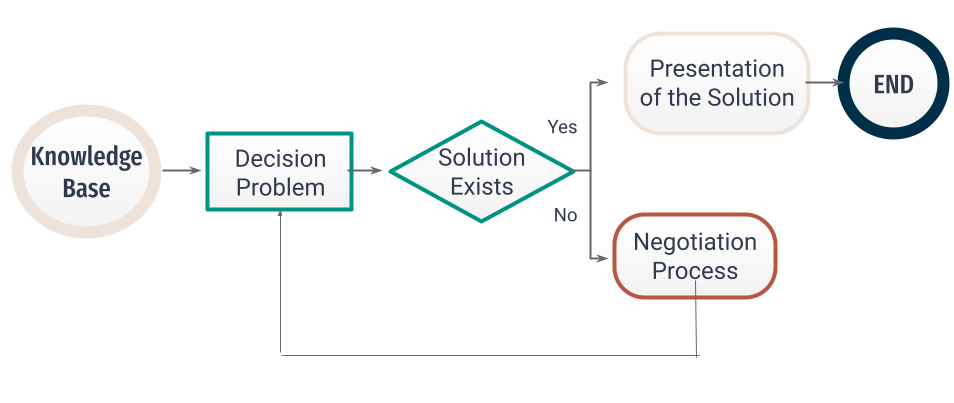
\includegraphics[width=0.95\textwidth]{./images/decision.png}
	\end{center}
	\caption{Role of Knowledge in decision making}\label{fig:decision}
\end{figure}

\chapter{Knowledge in Cognitive Systems}\label{Knowledge in Cognitive Systems}

\section{The Concept of Learning}\label{The Concept of Learning}
For a Cognitive System, the main aspect of knowledge gathering and it's
management boils down to it's learning. Learning is the most important aspect
of a Cognitive System. A Cognitive System which cannot learn from it's own
actions and the data which is constantly updated to it can not be helpful to
us. Just like how humans learn from their actions and develop changes within
their thought process according to the situation present in front of them, the
Cognitive System must be able to deal with the challenges and updations
regularly.

\section{Corpus Building}\label{Corpus Building}
Corpus refers to the \textbf{machine readable} format of the data provided. It
includes all the various types of data necessary for a Cognitive System for
working in a format which is easily identified by the system.

Corpus is extensively used by many experts of various fields as it helps in
Linguistic Analysis and various other research oriented tasks. Take for example
a medical professional(the analogies and examples of correlation between
Cognitive Systems and Healthcare will be encountered a lot in this chapter),
who wants to recommend medicines for his/her patients. If the professional has
access to the corpus, then it becomes easier to recommend new and effective
medicines and treatment to patients since the corpus provides access to the
various research advancements and discoveries to the experts.

Corpus also needs to be maintained in a proper fashion and has to be made in
such a way that it remains useful to experts after every iteration of updation.
If the new data added contains a lot of vague and unnecessary information, then
it makes the corpus less useful and overtime it will loose it's credibility and
will become obscure. On the other hand, if the data added is limiting it's full
potential of precise data, then it can not be used for Hypothesis Scoring and
will loose precious insights. The Machine Leaning of the Cognitive Systems will
depend upon the quality of the corpus provided.

A Cognitive System uses several layers of Analytical and Extraction Services
which act upon the data provided to the Cognitive System. These layers act as
an intermediary for the outside world and the working models of the Cognitive
System. They provide tools for representing data into ways which highlight the
properties.

Electronic Medical Records(EMR) are a good example, cause they provide the
experts with valuable information that may not be available to them through
sheer memory and personal experiences only. They also provide an apt
representation of the various methods and tools accessible to the experts.


Corpus Building also leads to various security issues as well. These include:-

\begin{itemize}
	\item The way data is added to the Cognitive Systems is usually through the ETL
	      method, i.e, \textbf{E}xtract-\textbf{T}ransform-\textbf{L}oad method, which
	      can lead to management and security risks.
\end{itemize}

\begin{itemize}
	\item Developers need to be certain about the compliance of data and metadata present
	      in the corpus.
\end{itemize}

\begin{itemize}
	\item The availability of tools does not relieve the developers from verification of
	      the data coming from various sources and to check it's authenticity.
\end{itemize}

\section{Introduction of Big Data in Cognitive Systems}\label{Big Data and Cognitive Systems}

With the advent of the internet and later all the new technological platforms,
the amount of data keeps on increasing. This data is very beneficial for the
Cognitive Systems, since it keeps it updated to the new trends and helps in
increasing it's efficiency, but the main issue arises with it's management.
This enormous data cannot be handled with the traditional methods of handling
conventional data.

This calls for devising new methods and techniques for handling such data and
this type of data is called \textbf{Big Data}.

Big Data already is and also will be an important aspect of Cognitive Computing
since we already live in an age where loads of data is being produced everyday,
either through social media apps, IoT and smart devices, legacy data, storage
units for Banking and Healthcare Sector, etc.

Big Data can be classified as :

\begin{itemize}
	\item Structured Data

	\item Unstructured Data

	\item Semi-Structured Data
\end{itemize}

These types of data constitute most of the data we deal with. For further
explaining Structured Data, here are it's few types:-

\begin{itemize}
	\item \textbf{Key-Value Pair}: Includes data that has a pointer(Key) and it's assigned dataset(Value). eg - XML Based documents and EDI Systems


	\item \textbf{Columnar Database}: Data which is stored in columns instead of rows, which makes it easier for reading and writing data on the disk. eg - HBase and Google's BigTable

	\item \textbf{Graph Database}: Data which is sotred in a single structure,i.e, Graph,which includes nodes and edges.eg - Neo4j
\end{itemize}

There are also several Data Services Tools which are helpful for the developers
in maintaining Cognitive Systems and it's Corpus. These include :-

\begin{itemize}
	\item ETL (Extract-Transform-Load) that is mainly used for Hadoop and it's features,
	      mainly for managing structured and unstructured data.

	\item Distributed File System, mainly used for managing data coming from varied
	      sources

	\item Coordination Services, used for taking leverage on distributed data.
\end{itemize}
